\documentclass[a4paper,11pt]{article}
\usepackage[utf8]{inputenc}
\usepackage{amsfonts}
\usepackage{graphicx}
%opening
\title{A spatial Poisson transmission model for Ebola (and other diseases)}
\author{Thibaut, Pierre, Anne, Nick G. and the Ebola team}

\begin{document}

\maketitle

\begin{center}
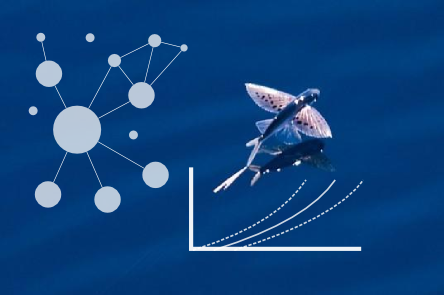
\includegraphics{figs/spatialPoisson} 
\end{center}

\begin{abstract}
The model is a meta-population model using a known (spatial) connectivity matrix between patches and a simple kernel to model dispersal. 
The model is based on incidence data, with only infected individuals being 
known.
Optionally, it can include infection from an unsampled reservoir.
Unlike \textit{outbreaker}, we are not trying to model individual ancestries, 
but merely dynamics within and between patches.
In its simplest form, the model has only two parameters and its likelihood can 
be computed very fast.
More complex extensions can allow for time-varying reproduction number, and/or 
time/spatially varying infection from the reservoir.
\end{abstract}

\newpage
%%%%%%%%%%%%%%%%%%%%%%%
%%%%%%%%%%%%%%%%%%%%%%%
\section{Notations}
%%%%%%%%%%%%%%%%%%%%%%%
%%%%%%%%%%%%%%%%%%%%%%%

\begin{itemize}
 \item $I_t^i$: observed incidence in patch $i$ at time $t$ (data)
 \item $N_t^i$: true, unobserved incidence in patch $i$ at time $t$ (augmented data)
 \item $I_t, N_t$: vectors of (observed, true) incidence of all patches
 \item $I,T$: matrix of observed / true incidence of all patches at all time steps $(I_t^1, \ldots, I_t^N)$
 \item $T$: the last date of the data
 \item $D_{ij}$: distance between $i$ and $j$
 \item $w(.)$: the known probability mass distribution of the generation time / serial interval
 \item $P$: number of patches in the model
 \item $n_t^i$: the number of infected individuals in patch $i$ at time $t$
 \item $d_{j\rightarrow i}$: intensity of dispersion from $j$ to $i$
 \item $\delta$: general dispersal parameter
 \item $\phi$: background force of infection
 \item $R$: the effective reproduction number
 \item $t_k$: the date of infection of individual $k$
 \item $f_\mathcal{P}(a,b)$: the Poisson density for $a$ observations and a rate $b$
 \item $k(c,d)$: a spatial kernel for a distance $c$ and a parameter $d$
\end{itemize}





%%%%%%%%%%%%%%%%%%%%%%%
%%%%%%%%%%%%%%%%%%%%%%%
\section{Model}
%%%%%%%%%%%%%%%%%%%%%%%
%%%%%%%%%%%%%%%%%%%%%%%

We want to sample from the posterior distribution proportional to:
\begin{equation}
 p(I, N, R, \phi, \delta, \omega) = p(I, N | R, \phi, \delta, \omega) p(R, \phi, \delta, \omega)
\end{equation}
which can be rewritten
\begin{equation}
\underbrace{p(I | N, \omega) p(N | R, \phi, \delta)}_{likelihood} 
\underbrace{ p(R) p(\phi) p(\delta) p(\omega)}_{priors} 
\end{equation}

The term $p(I | N, \omega)$ is the probability of the observed incidence given the true incidence $N$ and the reporting probability $\omega$.
It is computed as:

\begin{equation}
p(I | N, \omega) = \prod_{t}\prod_{i} f_\mathcal{B}(I_t^i, N_t^i, \omega)
\end{equation}
where $f_\mathcal{B}(x,a,b)$ is the Binomial p.m.f. for $x$ successes, $a$ draws and a probability $b$.
\\

The term $p(N | R, \phi, \delta)$ is the probability of the true incidence given the infectivity in the system and the spatial processes at play.
It is computed as:

\begin{equation}
p(N | R, \phi, \delta) = \prod_{t}\prod_{i} f_\mathcal{P}(N_t^i, \lambda_t^i)
\end{equation}
where $f_\mathcal{P}$ if the p.m.f of a Poisson distribution and $\lambda_t^i$ the force of infection towards patch $i$ and time $t$.
$\lambda_t^i$ is a sum over of the forces of infection of all patches towards $i$ (including $i \rightarrow i$). 
We note $\beta_t^i$ the force of infection coming from infected individuals in 
patch $i$ at time $t$, defined by the renewal equation:
\begin{equation}
 \beta_t^i = R \sum_{k=1}^{n_t^i} w(t - t_k)
\end{equation}
Where $R$ is the reproduction number. 
Note that we can easily turn it into a time-dependent term $R_t$, in which case 
we will have to assume i) a functional form or ii) $R_t$ constant 
between break-points. 
Similarly, it can be turned into a patch-specific $R_i$, in which case 
heterogeneity between patches can be modeled using a given distribution.
This can get more complicated quickly.
\\

The force of infection experienced by patch $i$ at time $t$ is then:
\begin{equation}
\lambda_t^i = \phi + \sum_{j=1}^P d_{j\rightarrow i} \beta_t^i
\end{equation}
where $d_{j\rightarrow i}$ is the diffusion from $j$ to $i$ defined by a kernel 
$k$:
\begin{equation}
d_{j\rightarrow i} = k(D_{ij}, \delta)
\end{equation}
where $D_{ij}$ is the known distance between $i$ and $j$ (which needs not be 
Euclidean or symmetric).
\\

%The likelihood of $I_t$, the incidence vector at time $t$, is defined as:
%\begin{equation}
%p(I_t | R, \delta) = \prod_{i=1}^P f_\mathcal{P}(I_t^i, \lambda_t^i)
%\end{equation}
%where $f_\mathcal{P}$ is the $pmf$ of a Poisson distribution.
%\\
%
%By extension, the likelihood for the entire data is:
%\begin{equation}
%p(I_1, \ldots, I_t | R, \delta) = \prod_{t=1}^T \prod_{i=1}^P 
%f_\mathcal{P}(I_t^i, \lambda_t^i)
%\end{equation}
%


%
%%%%%%%%%%%%%%%%%%%%%%%%
%%%%%%%%%%%%%%%%%%%%%%%%
%\section{Unobserved reservoir}
%%%%%%%%%%%%%%%%%%%%%%%%
%%%%%%%%%%%%%%%%%%%%%%%%
%
%So far the model assumes that all patches are known, and the connectivity 
%between the patches is known as well -- up to a dispersal parameter $\delta$.
%An unobserved reservoir (e.g. zoonotic cases) can be added using a few 
%assumptions. 
%To model the reservoir, we need to estimate the force of infection coming from 
%the reservoir to the different patches:
%\begin{equation}
%\phi_t^i = d_{res \rightarrow i} \beta_t^{res}
%\end{equation}
%
%We can make different assumptions on the two components, depending on whether 
%we are interested in modeling spatial or temporal heterogeneity.
%The simplest approach is to assume a constant 
%force of infection over time and equal across patches, in which case only one 
%additional parameter needs to be estimated.
%A more flexible approach would be to use a distribution of $\phi_t^i$ to 
%account for heterogeneity between patches.
%This is still a parsimonious approach in terms of parameters (typically 1-2 
%would be needed).

%
%
%%%%%%%%%%%%%%%%%%%%%%%%
%%%%%%%%%%%%%%%%%%%%%%%%
%\section{Complexity}
%%%%%%%%%%%%%%%%%%%%%%%%
%%%%%%%%%%%%%%%%%%%%%%%%
%
%In its simplest form, the model has 2 parameters without reservoir 
%($R$,$\delta$), and 3 with 
%reservoir ($R$,$\delta$,$\phi$).
%Likelihood computation will be fast, as we need only compute Poisson densities, 
%and no data augmentation.
%It can become much more complex with time-varying $R$ and time-varying, 
%spatially heterogeneous infection from the reservoir $\phi$.
%There will probably also be issues trying to estimate time-varying $R$ and 
%$\phi$, as the two effects would be largely confounded.
%

\end{document}
